\documentclass[tikz,border=4mm]{standalone}

\usepackage{pgfplots}
\pgfplotsset{compat=1.16}
\usetikzlibrary{arrows.meta,calc,decorations.pathreplacing,patterns}

\definecolor{lyso}{RGB}{195,55,45}
\definecolor{glass}{RGB}{45,155,120}
\definecolor{sipm}{RGB}{50,85,170}
\definecolor{sourcecol}{RGB}{230,160,55}
\definecolor{scattercol}{RGB}{210,115,45}
\definecolor{linegray}{RGB}{75,75,75}

\begin{document}
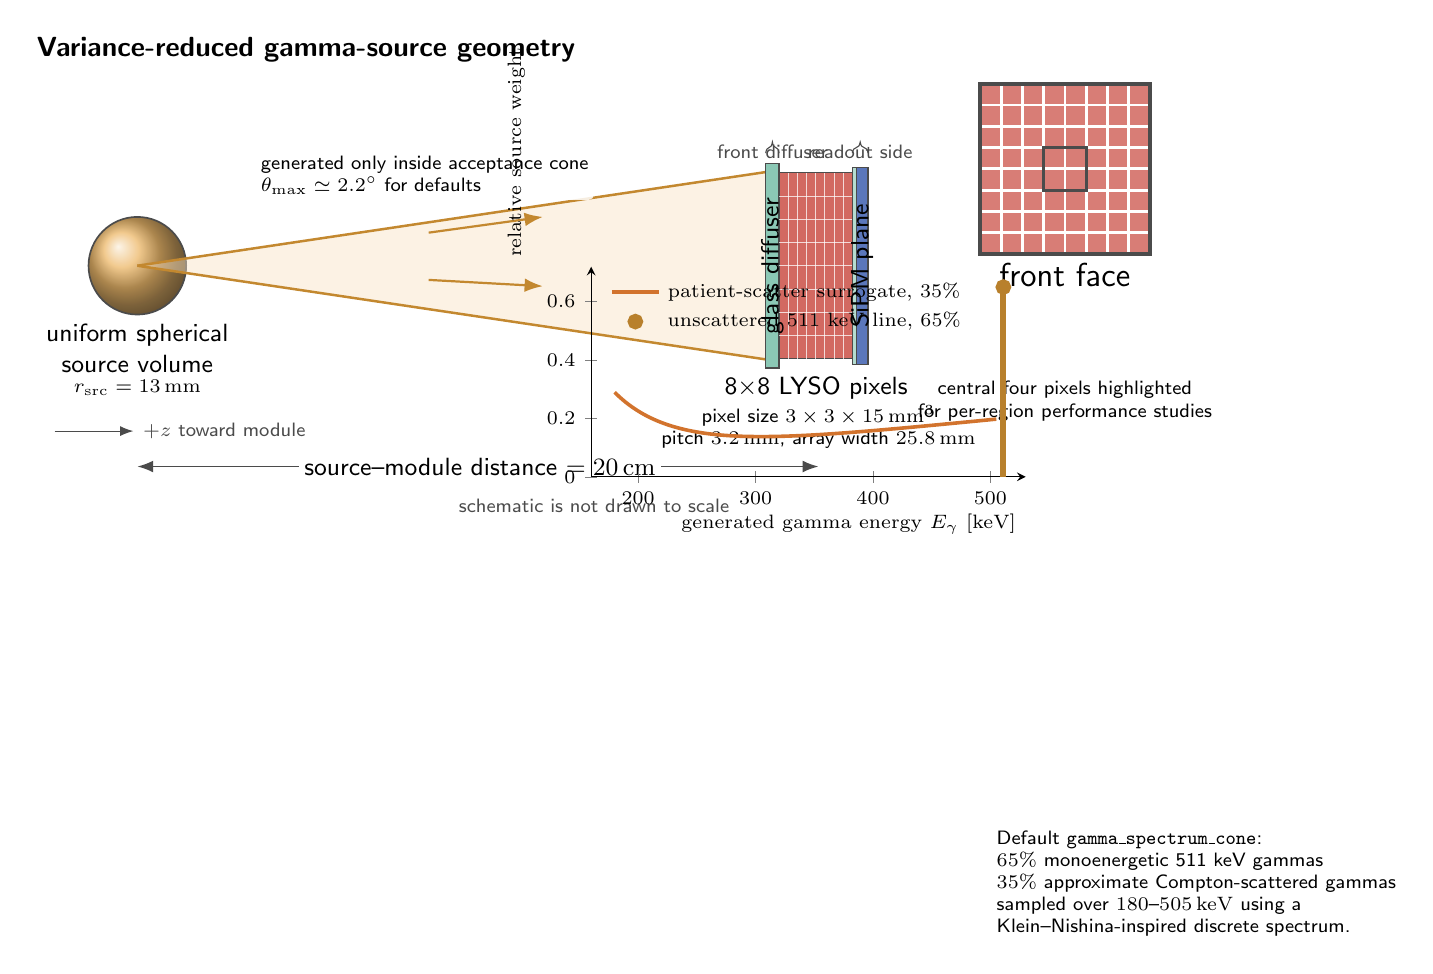
\begin{tikzpicture}[
    >=Latex,
    font=\sffamily,
    label/.style={font=\sffamily\small},
    note/.style={font=\sffamily\scriptsize, align=left},
    material/.style={draw=linegray, line width=0.45pt},
]

% ----------------------------------------------------------------------
% Geometry schematic
% ----------------------------------------------------------------------
\node[anchor=west, font=\sffamily\bfseries] at (-7.1,2.75) {Variance-reduced gamma-source geometry};

% Coordinates are schematic: the 20 cm separation is compressed.
\coordinate (S) at (-5.7,0.0);
\coordinate (Mfront) at (2.35,0.0);
\coordinate (Mcentre) at (2.95,0.0);

% Source sphere
\shade[ball color=sourcecol!80, opacity=0.95] (S) circle (0.62);
\draw[linegray, line width=0.6pt] (S) circle (0.62);
\node[label, align=center] at (-5.7,-1.05) {uniform spherical\\source volume};
\node[note, align=center] at (-5.7,-1.55) {$r_{\rm src}=13\,{\rm mm}$};

% Cone of generated gammas
\fill[sourcecol!30, opacity=0.45] (S) -- (2.35,1.20) -- (2.35,-1.20) -- cycle;
\draw[sourcecol!85!black, line width=0.9pt] (S) -- (2.35,1.20);
\draw[sourcecol!85!black, line width=0.9pt] (S) -- (2.35,-1.20);
\draw[->, sourcecol!85!black, line width=0.8pt] (-2.0,0.42) -- (-0.55,0.62);
\draw[->, sourcecol!85!black, line width=0.8pt] (-2.0,-0.18) -- (-0.55,-0.26);
\node[note, fill=white, fill opacity=0.85, text opacity=1, rounded corners=2pt, inner sep=2pt]
  at (-2.05,1.15) {generated only inside acceptance cone\\$\theta_{\rm max}\simeq2.2^\circ$ for defaults};

% Module side view: front glass, LYSO array, back glass, SiPM
\draw[material, fill=glass!55] (2.28,-1.30) rectangle (2.45,1.30);
\draw[material, fill=lyso!75] (2.45,-1.18) rectangle (3.38,1.18);
\draw[material, fill=glass!35] (3.38,-1.25) rectangle (3.43,1.25);
\draw[material, fill=sipm!80] (3.43,-1.25) rectangle (3.58,1.25);
\draw[linegray, line width=0.45pt] (2.45,-1.18) rectangle (3.38,1.18);
\foreach \y in {-0.885,-0.59,-0.295,0,0.295,0.59,0.885} {
  \draw[white, opacity=0.75, line width=0.25pt] (2.45,\y) -- (3.38,\y);
}
\foreach \x in {2.566,2.682,2.798,2.914,3.030,3.146,3.262} {
  \draw[white, opacity=0.75, line width=0.25pt] (\x,-1.18) -- (\x,1.18);
}
\node[label, rotate=90] at (2.365,0) {glass diffuser};
\node[label] at (2.92,-1.55) {8$\times$8 LYSO pixels};
\node[label, rotate=90] at (3.505,0) {SiPM plane};
\node[note, align=center] at (2.95,-2.05)
  {pixel size $3\times3\times15\,{\rm mm^3}$\\pitch $3.2\,{\rm mm}$, array width $25.8\,{\rm mm}$};

% Reflector note
\draw[decorate, decoration={brace, amplitude=4pt}, linegray] (2.28,1.43) -- (2.45,1.43)
  node[midway, yshift=0.35, note] {front diffuser};
\draw[decorate, decoration={brace, amplitude=4pt}, linegray] (3.38,1.43) -- (3.58,1.43)
  node[midway, yshift=0.35, note] {readout side};

% Distance annotation
\draw[<->, linegray, line width=0.6pt] ($(S)+(0,-2.55)$) -- ($(Mcentre)+(0,-2.55)$);
\node[label, fill=white, inner sep=2pt] at (-1.35,-2.55)
  {source--module distance $=20\,{\rm cm}$};
\node[note, text=linegray] at (0.1,-3.05) {schematic is not drawn to scale};

% Axis arrow
\draw[->, linegray] (-6.75,-2.1) -- (-5.75,-2.1) node[right, note] {$+z$ toward module};

% Face-on pixel-array inset
\begin{scope}[shift={(5.0,0.15)}, scale=0.27]
  \draw[material, fill=lyso!65] (0,0) rectangle (8,8);
  \foreach \i in {1,...,7} {
    \draw[white, line width=1.0pt] (\i,0) -- (\i,8);
    \draw[white, line width=1.0pt] (0,\i) -- (8,\i);
  }
  \draw[linegray, line width=1.4pt] (0,0) rectangle (8,8);
  \draw[linegray, line width=1.0pt] (3,3) rectangle (5,5);
  \node[font=\sffamily\large] at (4,-1.0) {front face};
\end{scope}
\node[note, align=center] at (6.08,-1.72)
  {central four pixels highlighted\\for per-region performance studies};

% ----------------------------------------------------------------------
% Energy spectrum inset
% ----------------------------------------------------------------------
\begin{axis}[
    at={(4.25,-3.25)},
    anchor=north west,
    width=7.1cm,
    height=4.25cm,
    xmin=160, xmax=530,
    ymin=0, ymax=0.72,
    axis lines=left,
    xlabel={generated gamma energy $E_\gamma$ [keV]},
    ylabel={relative source weight},
    xlabel style={at={(axis description cs:1.0,-0.13)}, anchor=north east},
    ylabel style={at={(axis description cs:-0.13,1.0)}, anchor=south west},
    tick label style={font=\scriptsize},
    label style={font=\scriptsize},
    legend style={font=\scriptsize, draw=none, fill=none, at={(0.02,0.98)}, anchor=north west},
]
  % Approximate Klein--Nishina transformed scattered spectrum.
  \addplot[scattercol, line width=1.3pt, domain=180:505, samples=140]
    {0.10*((x/511)+(511/x)-(1-(2-511/x)^2))};
  \addlegendentry{patient-scatter surrogate, 35\%}

  \addplot[ycomb, sourcecol!80!black, line width=2.2pt, mark=*, mark size=1.7pt]
    coordinates {(511,0.65)};
  \addlegendentry{unscattered 511 keV line, 65\%}
\end{axis}
\node[note, align=left] at (7.75,-7.85)
  {Default \texttt{gamma\_spectrum\_cone}:\\
   $65\%$ monoenergetic 511 keV gammas\\
   $35\%$ approximate Compton-scattered gammas\\
   sampled over $180$--$505\,{\rm keV}$ using a\\
   Klein--Nishina-inspired discrete spectrum.};

\end{tikzpicture}
\end{document}
